\section{Durchführung}
\label{sec:durchführung}

Abbildung~\ref{fig:aufbau} zeigt den wesentlichen Teil des Versuchaufbaus. Die
von der $\ce{^{137}Cs}$ Quelle ausgehende $\gamma$-Strahlung wird durch
Bleiblöcke zu großen Teilen abgeschirmt. Nur in Richtung eines Detektors wird
die Strahlung über eine Bleiblende nutzbar gemacht. Bei dem Detektor handelt es
sich um einen Szintillationsdetektr, der als szintillierendes Material
Natriumiodid (NaI) verwendet. Trifft $\gamma$-Strahlung auf das Material, werden
dessen Moleküle angeregt und emittieren Photonen. Die Detektion dieser Photon
erfolgt durch einen Photomultplier, der gemäß der Anzahl eintreffender Photonen
ein elektrisches Signal entsprechender Stärke an einen Multichannelanalyzer
weitergibt. Dieser histogrammiert die eintreffenden Signale an Hand ihrer
Impulshöhe. Die Ausgabe erfolgt über einen angeschlossenen Computer und ein
entsprechendes Analyseprogramm. Als zu untersuchende Objekte werden verschiedene
Würfel in den Strahlgang gebracht. Auf einer entsprechenden Halterung sind die
Würfel horizontal verschiebar und senkrecht zur Horizontalen drehbar gelagert.

\begin{figure}
  \centering
  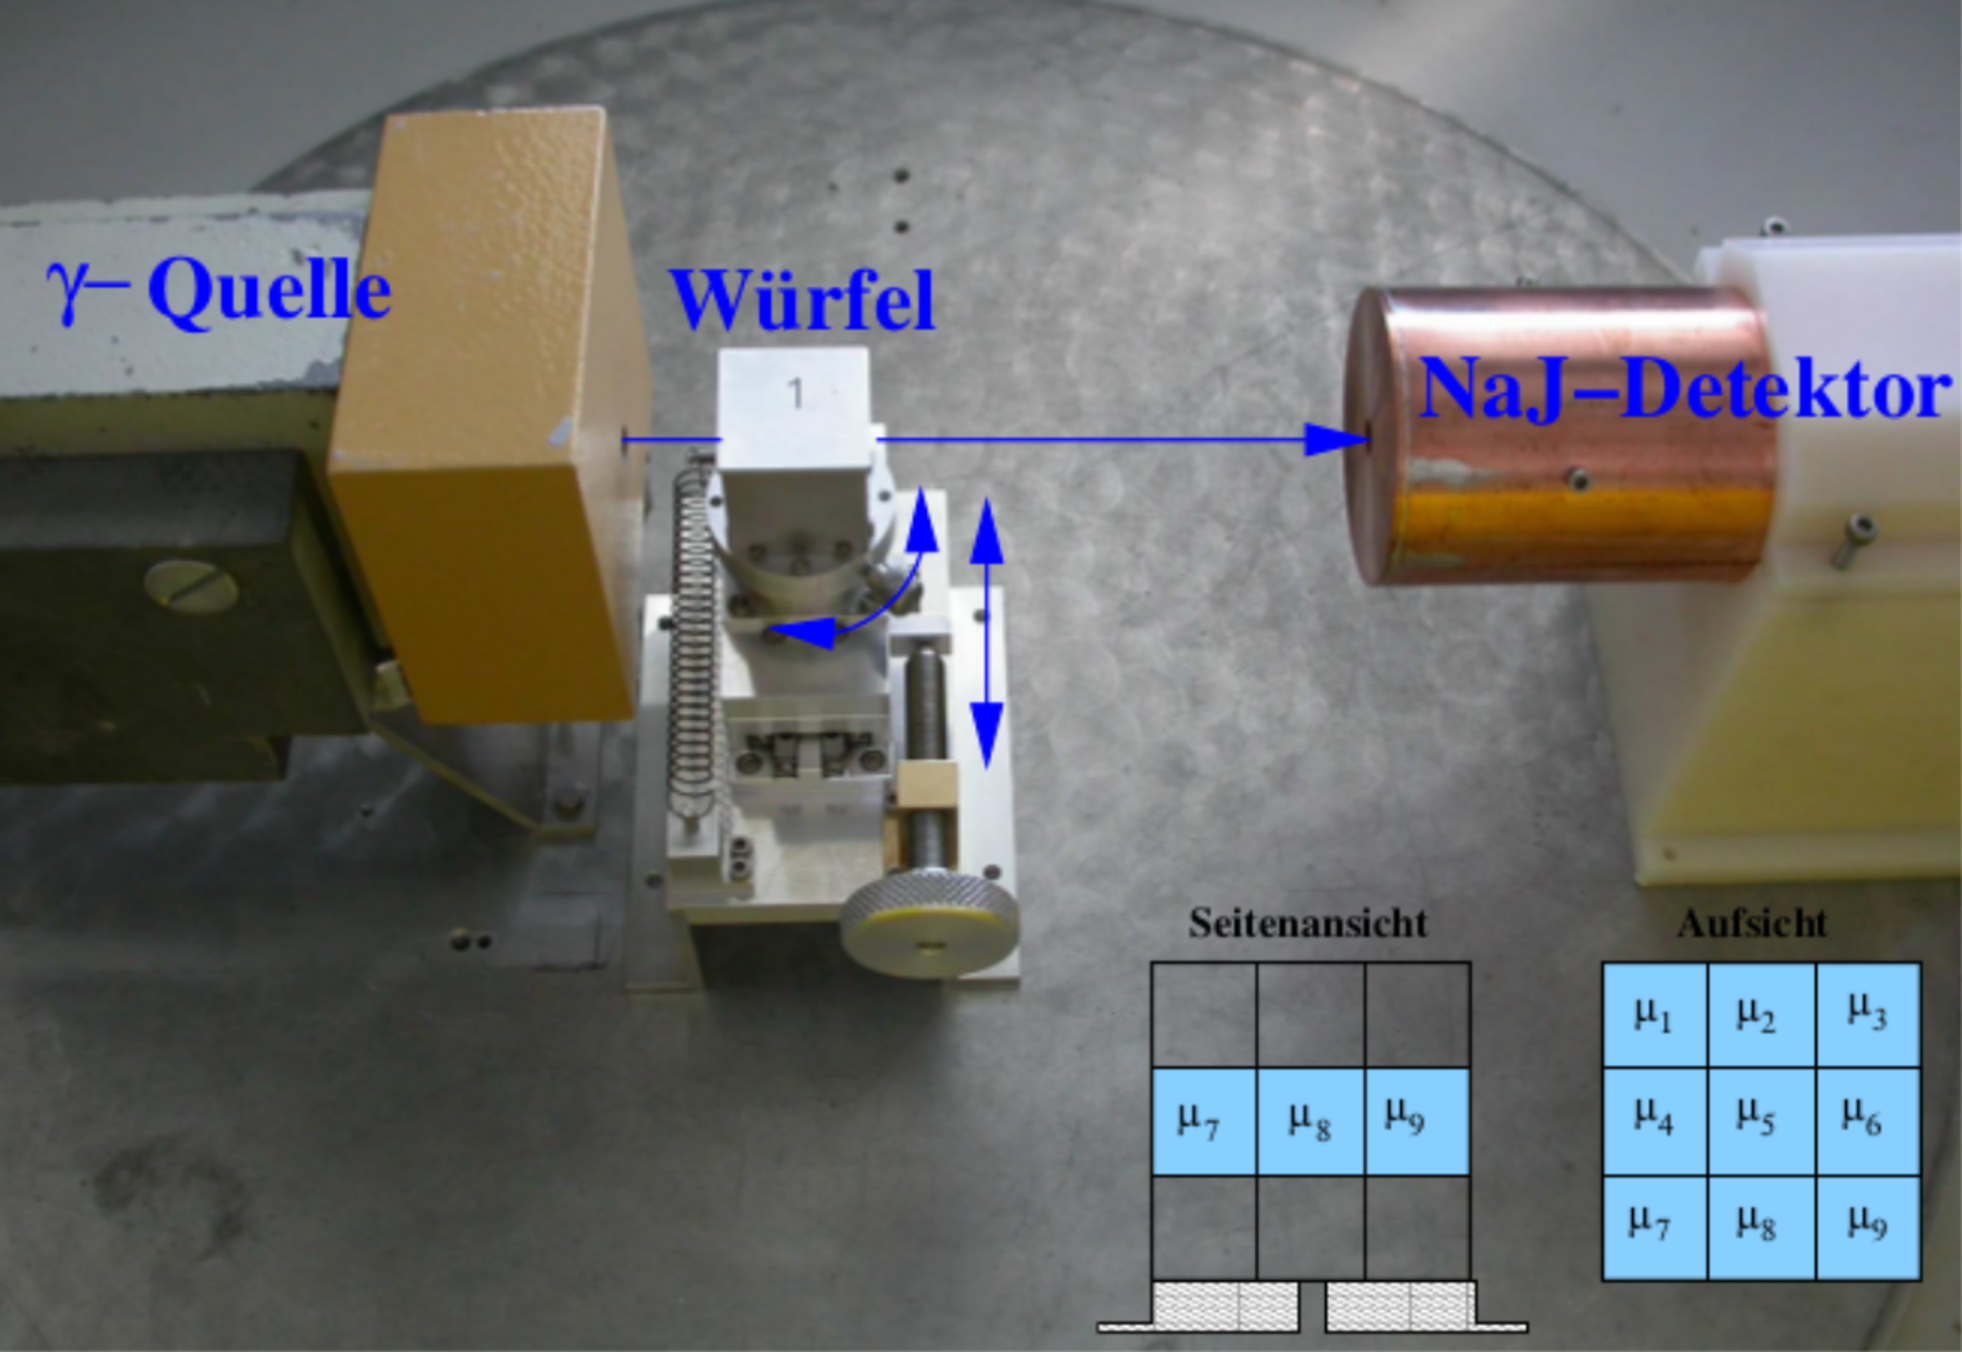
\includegraphics[width=0.7\textwidth]{figures/aufbau.pdf}
  \caption{Versuchsaufbau mit zu untersuchendem Würfel, einem 
  Natriumiodid-Detektor und einer $\ce{^{137}Cs}$ Quelle. Die umfangreiche
  Bleiabschirmung ist hier nicht zu sehen.}
  \label{fig:aufbau}
\end{figure}

Insgesamt werden fünf Messreihen durchgeführt. Zunächst wird eine Messung ohne
Würfel im Strahlgang durchgeführt (Nullmessung). Danach folgen Messungen mit
einem leeren Würfel (Würfel 1) (d.h. nur die Aluminiumummantelung befindet sich
im Strahlgang) für fünf verschiedene Ausrichtungen des Würfels. Sowohl für die
Nullmessung, als auch für die Leermessung wird neben der Anzahl an gezählten
Ereignissen auch das Strahlungsspektrum aufgenommen. Es folgen Messungen für die
Würfel 2 und 3 mit jeweils vier Würfelausrichtungen, wobei bekannt ist, dass
Würfel 2 vollständig aus Aluminium und Würfel 3 vollständig aus Blei besteht.
Abschließend wird Würfel 5 als ein Würfel mit unbekannter Zusammensetzung aus
allen zwölf Richtungen gemäß Abbilung~\ref{fig:projektionen} vermessen.
